%%%%%%%%%%%%%%%%%%%%%%%%%%%%%%%%%%%%%%%%%
% Short Sectioned Assignment
% LaTeX Template
% Version 1.0 (5/5/12)
%
% This template has been downloaded from:
% http://www.LaTeXTemplates.com
%
% Original author:
% Frits Wenneker (http://www.howtotex.com)
%
% License:
% CC BY-NC-SA 3.0 (http://creativecommons.org/licenses/by-nc-sa/3.0/)
%
%%%%%%%%%%%%%%%%%%%%%%%%%%%%%%%%%%%%%%%%%

%----------------------------------------------------------------------------------------
%	PACKAGES AND OTHER DOCUMENT CONFIGURATIONS
%----------------------------------------------------------------------------------------

\documentclass[paper=a4, fontsize=11pt]{scrartcl} % A4 paper and 11pt font size

\usepackage[T1]{fontenc} % Use 8-bit encoding that has 256 glyphs
\usepackage{fourier} % Use the Adobe Utopia font for the document - comment this line to return to the LaTeX default
\usepackage[english]{babel} % English language/hyphenation
\usepackage{amsmath,amsfonts,amsthm} % Math packages

\usepackage{lipsum} % Used for inserting dummy 'Lorem ipsum' text into the template

\usepackage{sectsty} % Allows customizing section commands
\allsectionsfont{\centering \normalfont\scshape} % Make all sections centered, the default font and small caps

\usepackage{fancyhdr} % Custom headers and footers

% use for graph
\usepackage{graphicx} 
\usepackage{subfigure}
\usepackage{caption}
\usepackage{float} 

\pagestyle{fancyplain} % Makes all pages in the document conform to the custom headers and footers
\fancyhead{} % No page header - if you want one, create it in the same way as the footers below
\fancyfoot[L]{} % Empty left footer
\fancyfoot[C]{} % Empty center footer
\fancyfoot[R]{\thepage} % Page numbering for right footer
\renewcommand{\headrulewidth}{0pt} % Remove header underlines
\renewcommand{\footrulewidth}{0pt} % Remove footer underlines
\setlength{\headheight}{13.6pt} % Customize the height of the header

\numberwithin{equation}{section} % Number equations within sections (i.e. 1.1, 1.2, 2.1, 2.2 instead of 1, 2, 3, 4)
\numberwithin{figure}{section} % Number figures within sections (i.e. 1.1, 1.2, 2.1, 2.2 instead of 1, 2, 3, 4)
\numberwithin{table}{section} % Number tables within sections (i.e. 1.1, 1.2, 2.1, 2.2 instead of 1, 2, 3, 4)

\setlength\parindent{0pt} % Removes all indentation from paragraphs - comment this line for an assignment with lots of text

%----------------------------------------------------------------------------------------
%	TITLE SECTION
%----------------------------------------------------------------------------------------

\newcommand{\horrule}[1]{\rule{\linewidth}{#1}} % Create horizontal rule command with 1 argument of height

\title{	
\normalfont \normalsize 
\textsc{University College cork} \\ [25pt] % Your university, school and/or department name(s)
\horrule{0.5pt} \\[0.4cm] % Thin top horizontal rule
\huge The ethical issues in the use of AI in healthcare \\ % The assignment title
\horrule{2pt} \\[0.5cm] % Thick bottom horizontal rule
}

\author{Kai Deng} % Your name

\date{\normalsize\today} % Today's date or a custom date


\begin{document}
\maketitle % Print the title

%----------------------------------------------------------------------------------------
%	PROBLEM 1
%----------------------------------------------------------------------------------------

\section{Introduction}

In the 21st century, advancements in theory and computational power have rapidly propelled 
artificial intelligence (AI), especially in healthcare, drawing significant investments (see Figures 1.1 and 1.2). 
Proponents believe AI can enhance diagnostic accuracy, extend care to remote areas, and save doctors' 
time for more patient interaction \cite{frostPublicViewsEthical2022}. However, AI's potential to worsen 
health disparities due to biases has sparked ethical concerns about privacy, data ownership, biased system risks, 
and lack of human oversight \cite{onianiAdoptingExpandingEthical2023, katiraiEthicsAdvancingArtificial2023}. 
This text will explore these issues' origins and solutions.

\begin{figure}[H]
    \centering
    \begin{minipage}[t]{0.48\linewidth}
        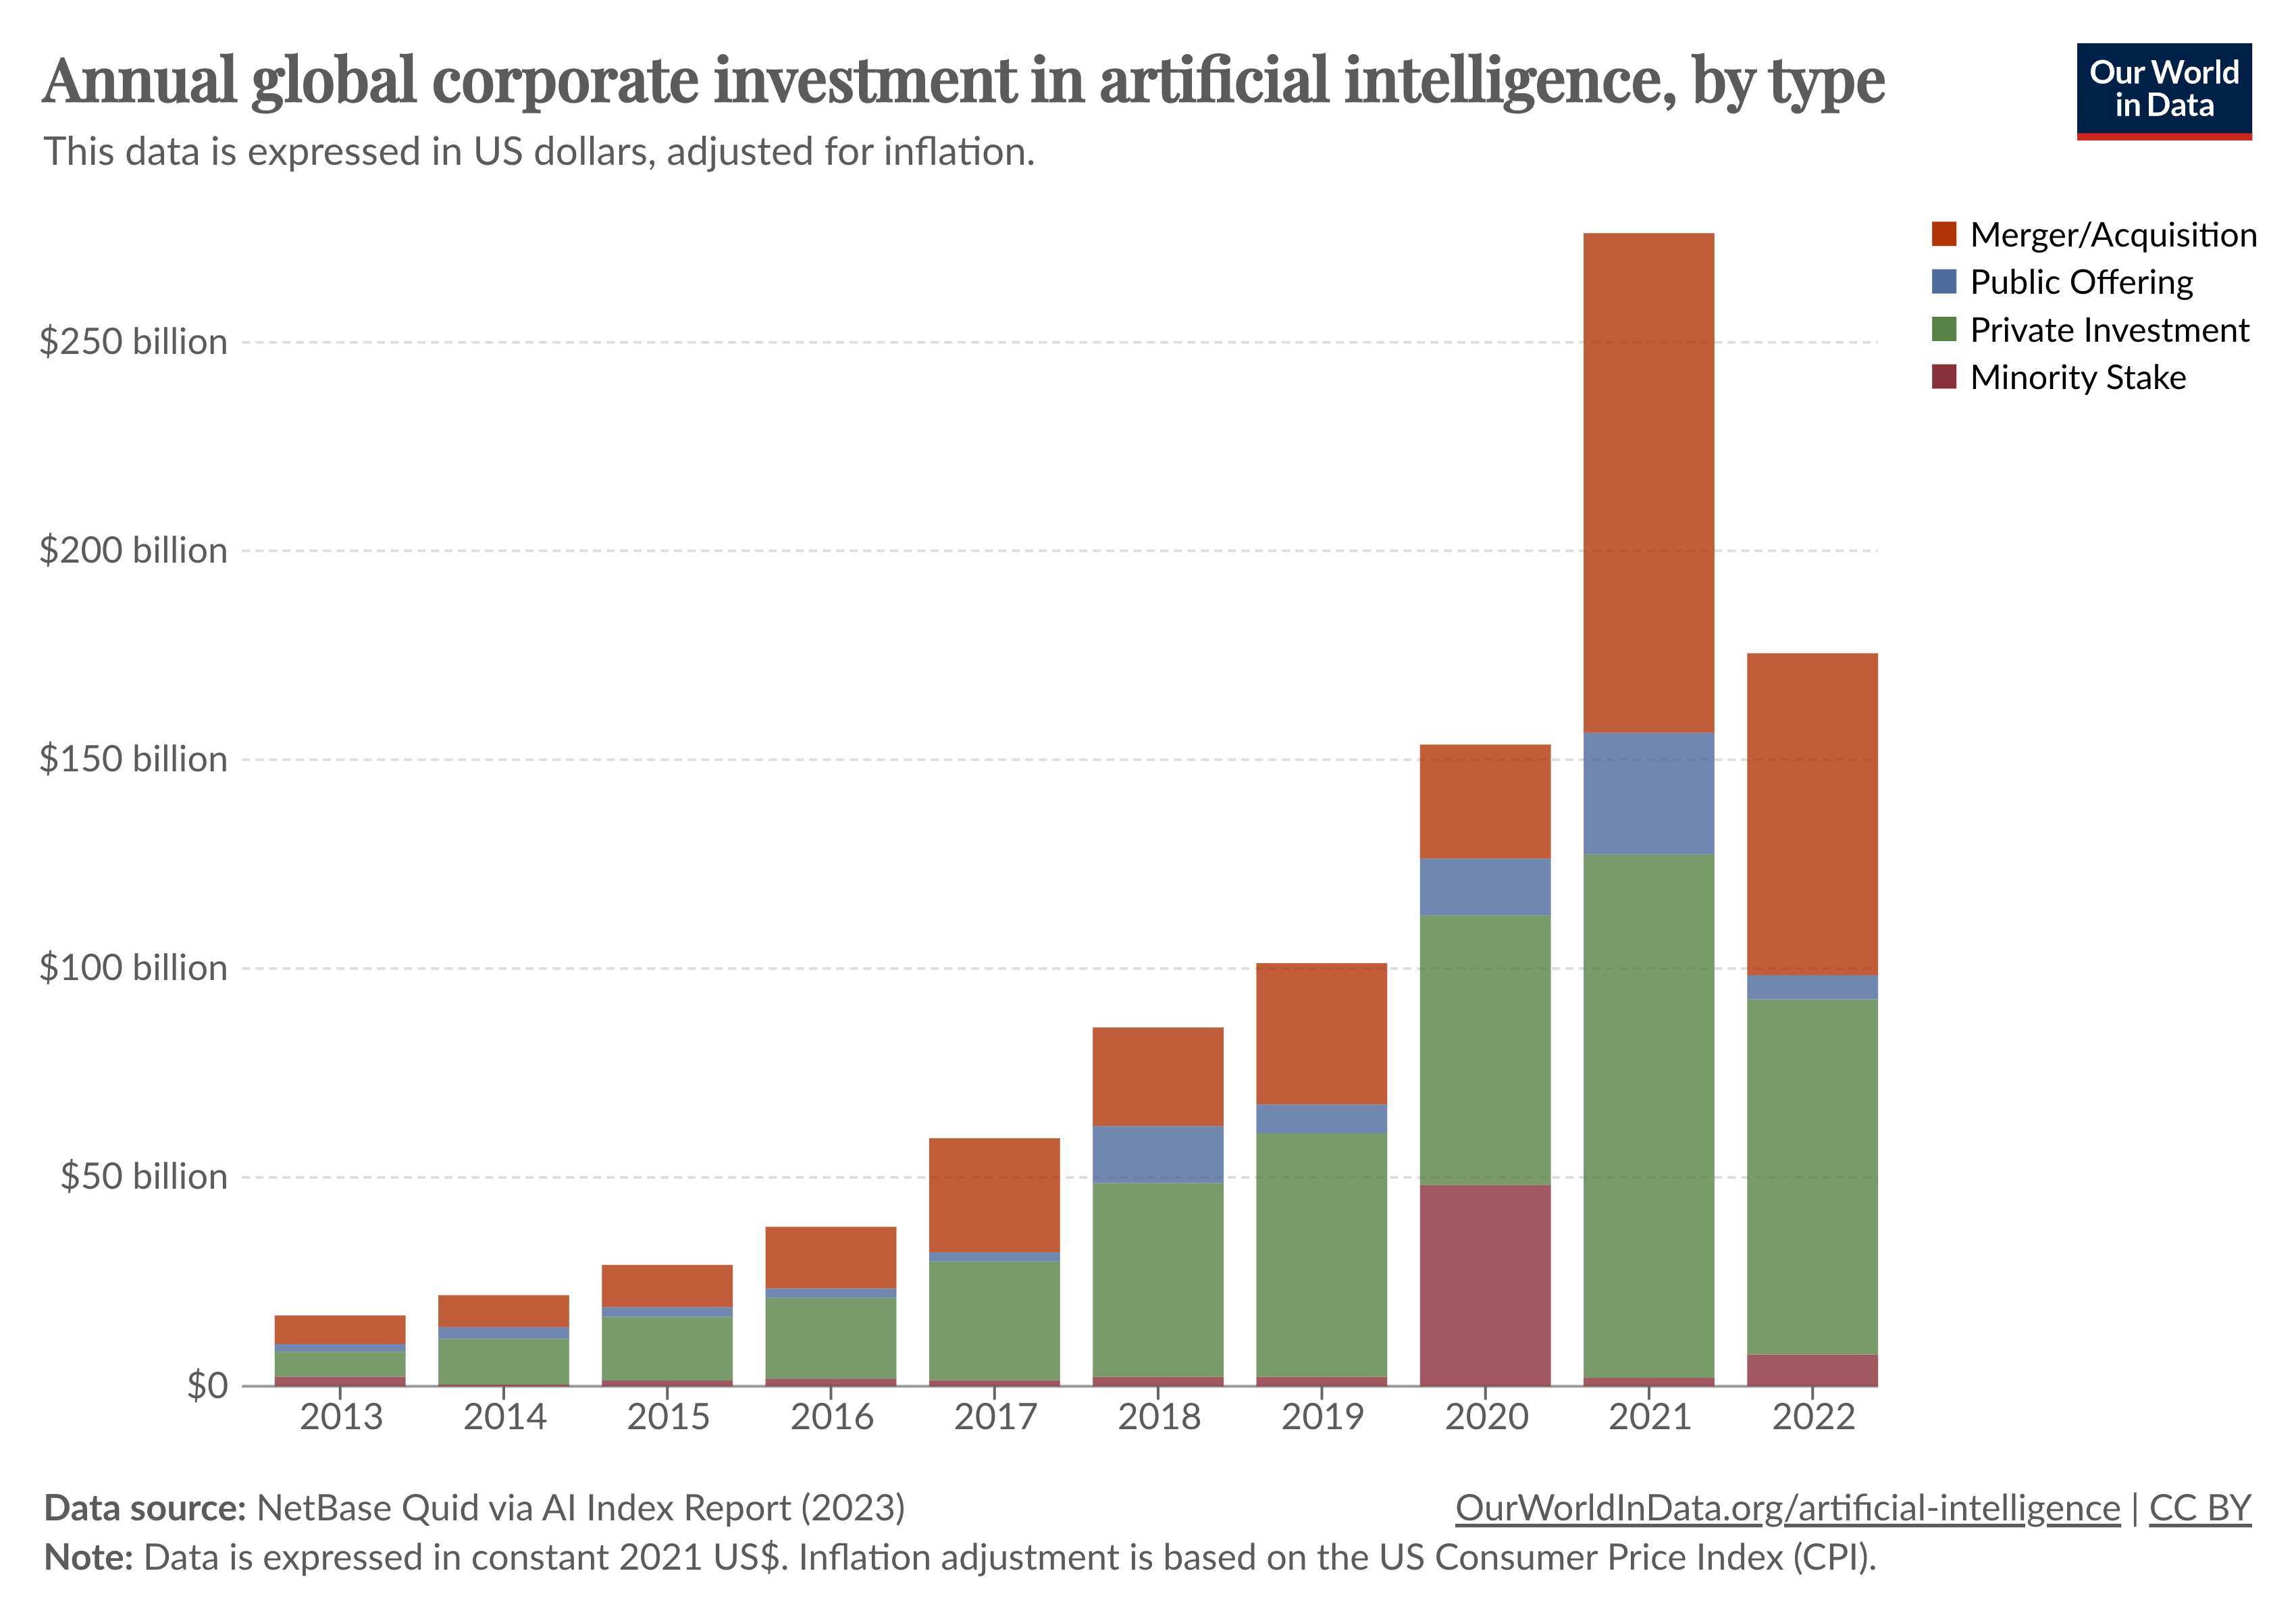
\includegraphics[width=\linewidth]{./data/investment_by_type.png}
        \caption{Annual investment in AI by type}
        \label{fig:investment}
    \end{minipage}\hfill
    \begin{minipage}[t]{0.48\linewidth}
        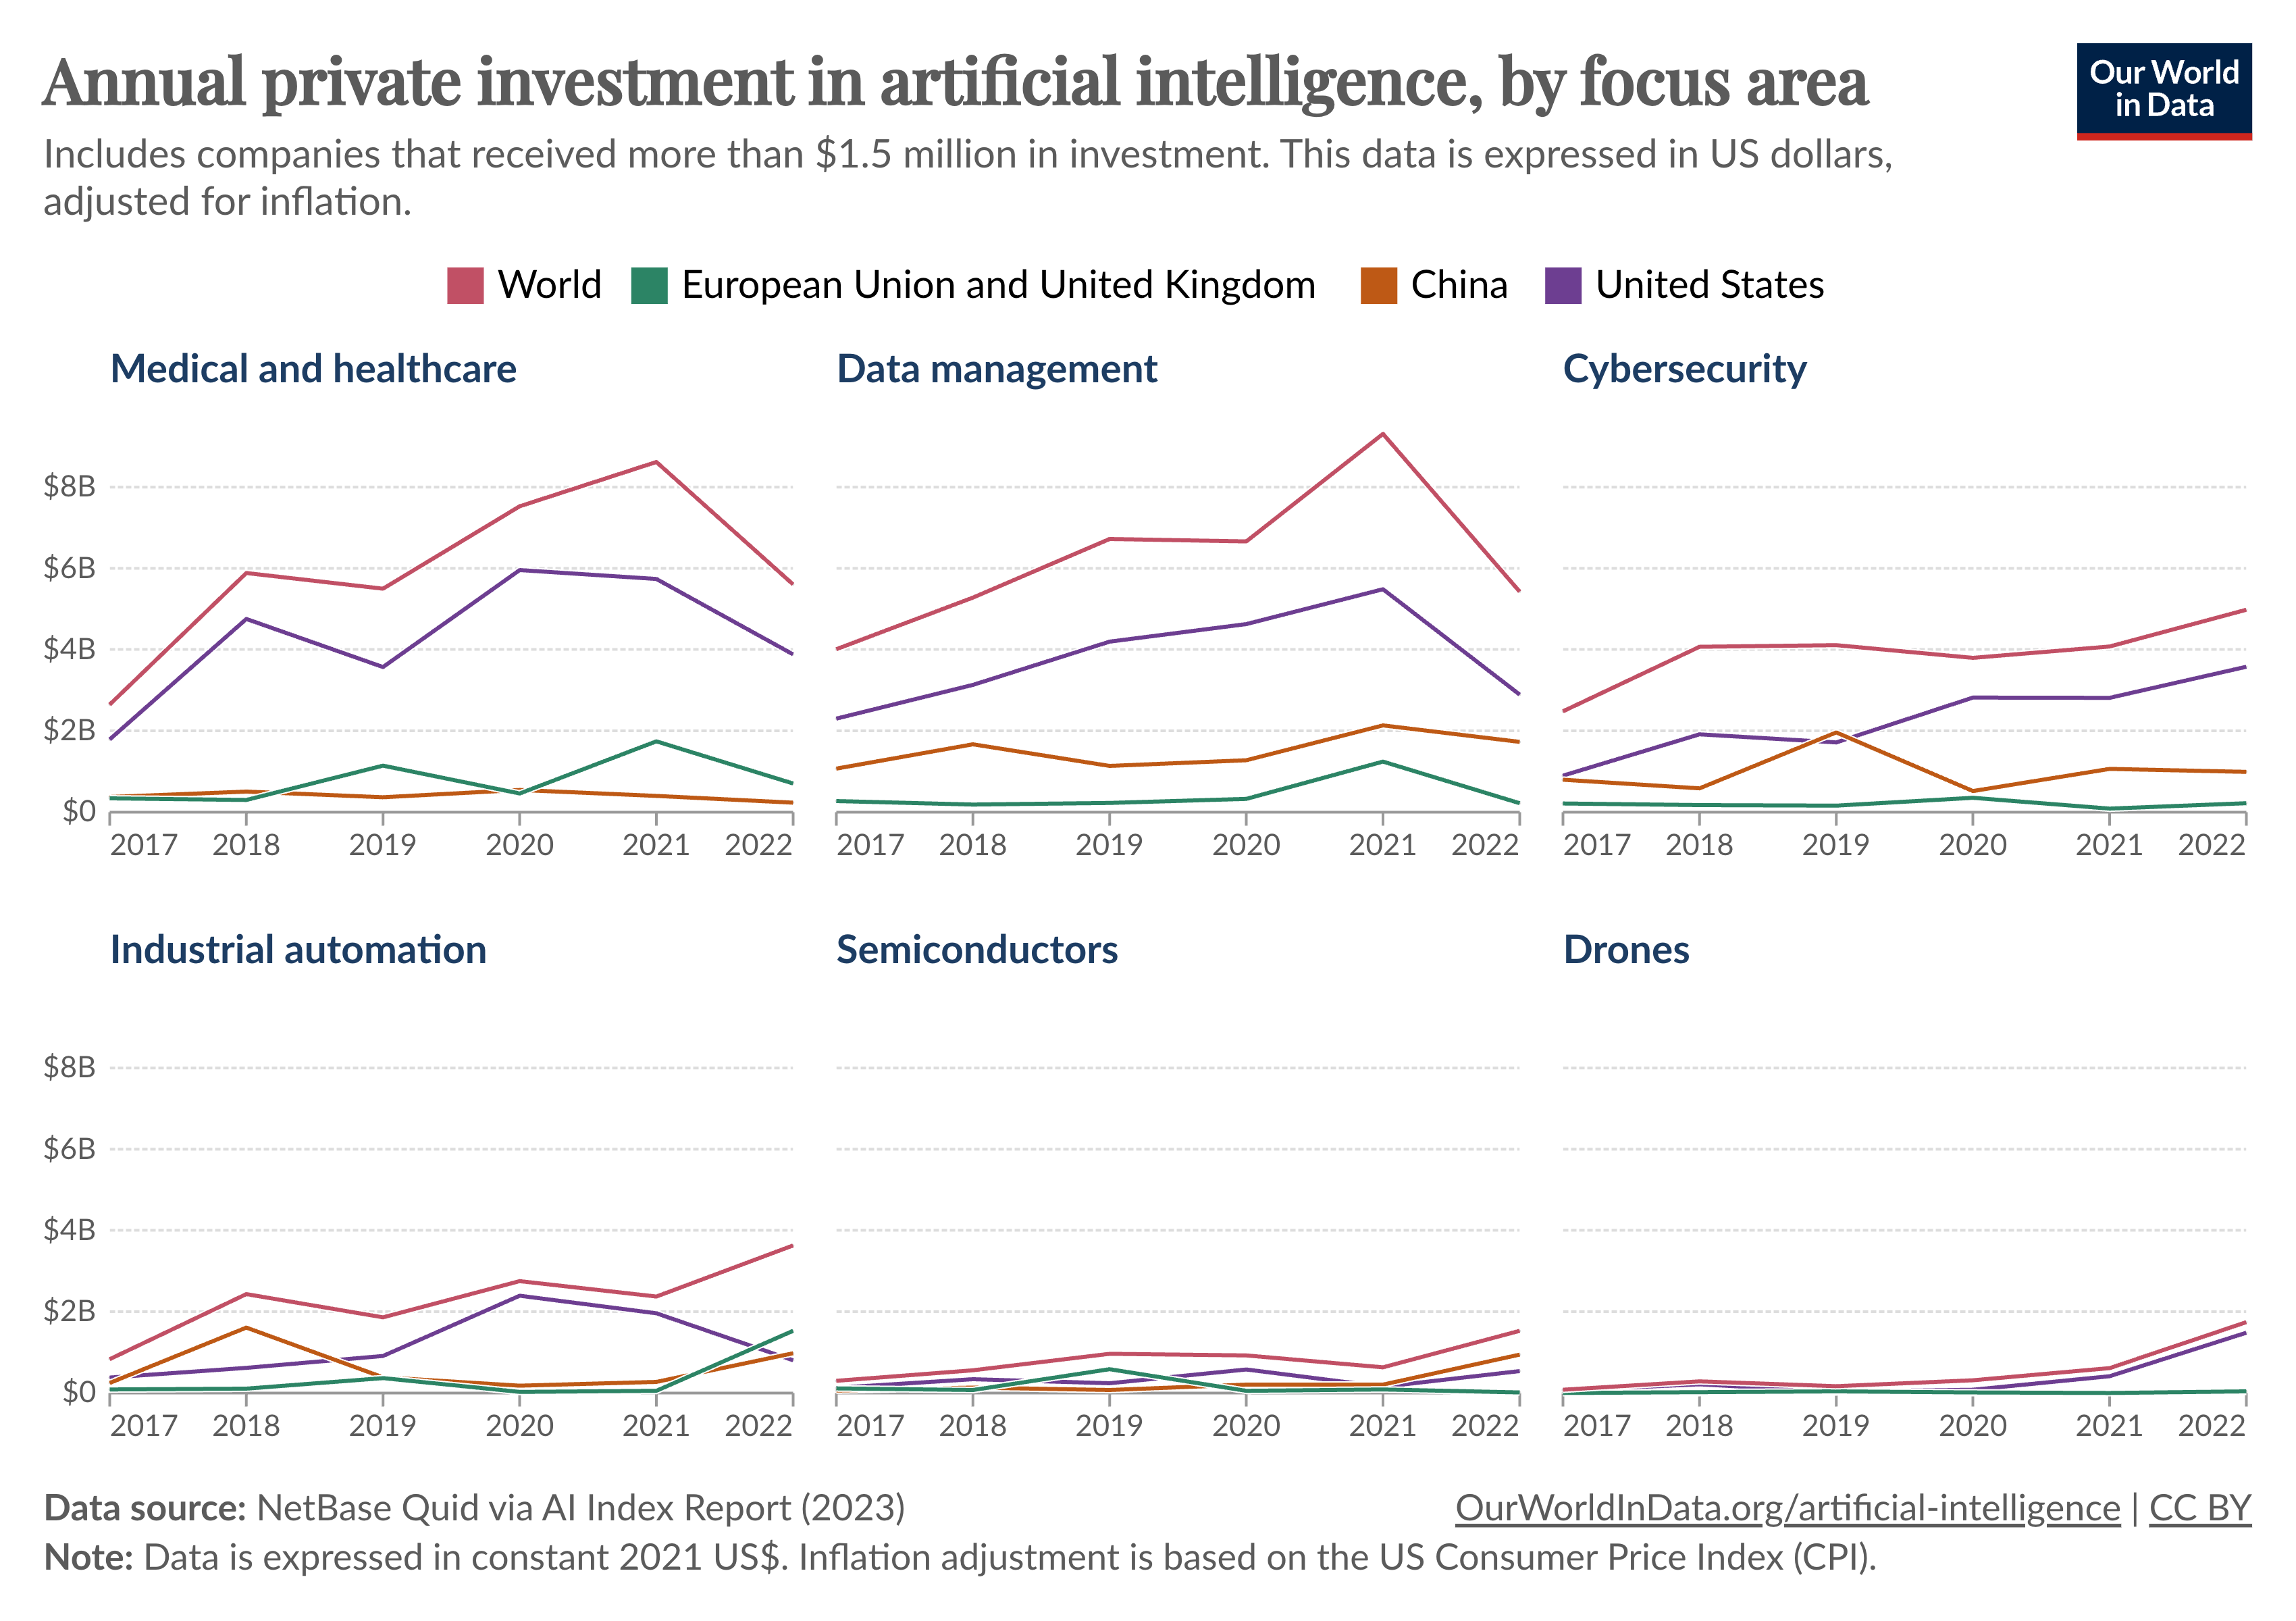
\includegraphics[width=\linewidth]{./data/investment_by_area.png}
        \caption{Annual investment in AI by area}
        \label{fig:views_ai_impact}
    \end{minipage}
\end{figure}



\section{section1}
% Public may be both benificiaries of new HCAI technologies and the greatest sufferers of AI-related harms. The result highlight that there are still noticeable concerns about 
% implementing HCAI in diagnostics and treatment recommendations for patients eith both acute and chronic illnesses, even if these tools are used as a recommendation system under the 
% physician experience and wisdom. Individuals may still not be ready to accept and use HCAI \cite{esmaeilzadehPatientsPerceptionsHuman2021}. Patients and publics are important voices In
% developing effective and ethical AI governance, but engaging patients and pbulics meanigfully in research about ethical HCAI is challenging. Most people have no first hand experience with HCAI,
% and some are unfamiliar with the concept of AI in general, Pulics may have limited understaing of how HCAI may be implemented and limited knowledge about the potential wrongs and harms that coudld
% arise from implementing HCAI \cite{frostPublicViewsEthical2022}, which means The public, as an actor, has yet to become more aware of privacy, data ownership, and human rights.

The public stands to gain from new HCAI technologies but also faces the highest risk of 
AI-related issues. Concerns persist around HCAI's role in diagnosing and suggesting treatments 
for both acute and chronic conditions, despite physician oversight. Many are hesitant to embrace HCAI \cite{esmaeilzadehPatientsPerceptionsHuman2021}. 
Engaging patients and the wider public in ethical HCAI discussions is crucial yet challenging. 
Most lack direct HCAI experience or even a basic understanding of AI. Their limited insight into HCAI's 
application and the potential for harm highlights the need for greater awareness around privacy, data rights, 
and human rights \cite{frostPublicViewsEthical2022}, emphasizing the importance of informed public participation in AI governance.



\begin{figure}[htbp]
    \centering
    \begin{minipage}[t]{0.48\linewidth}
        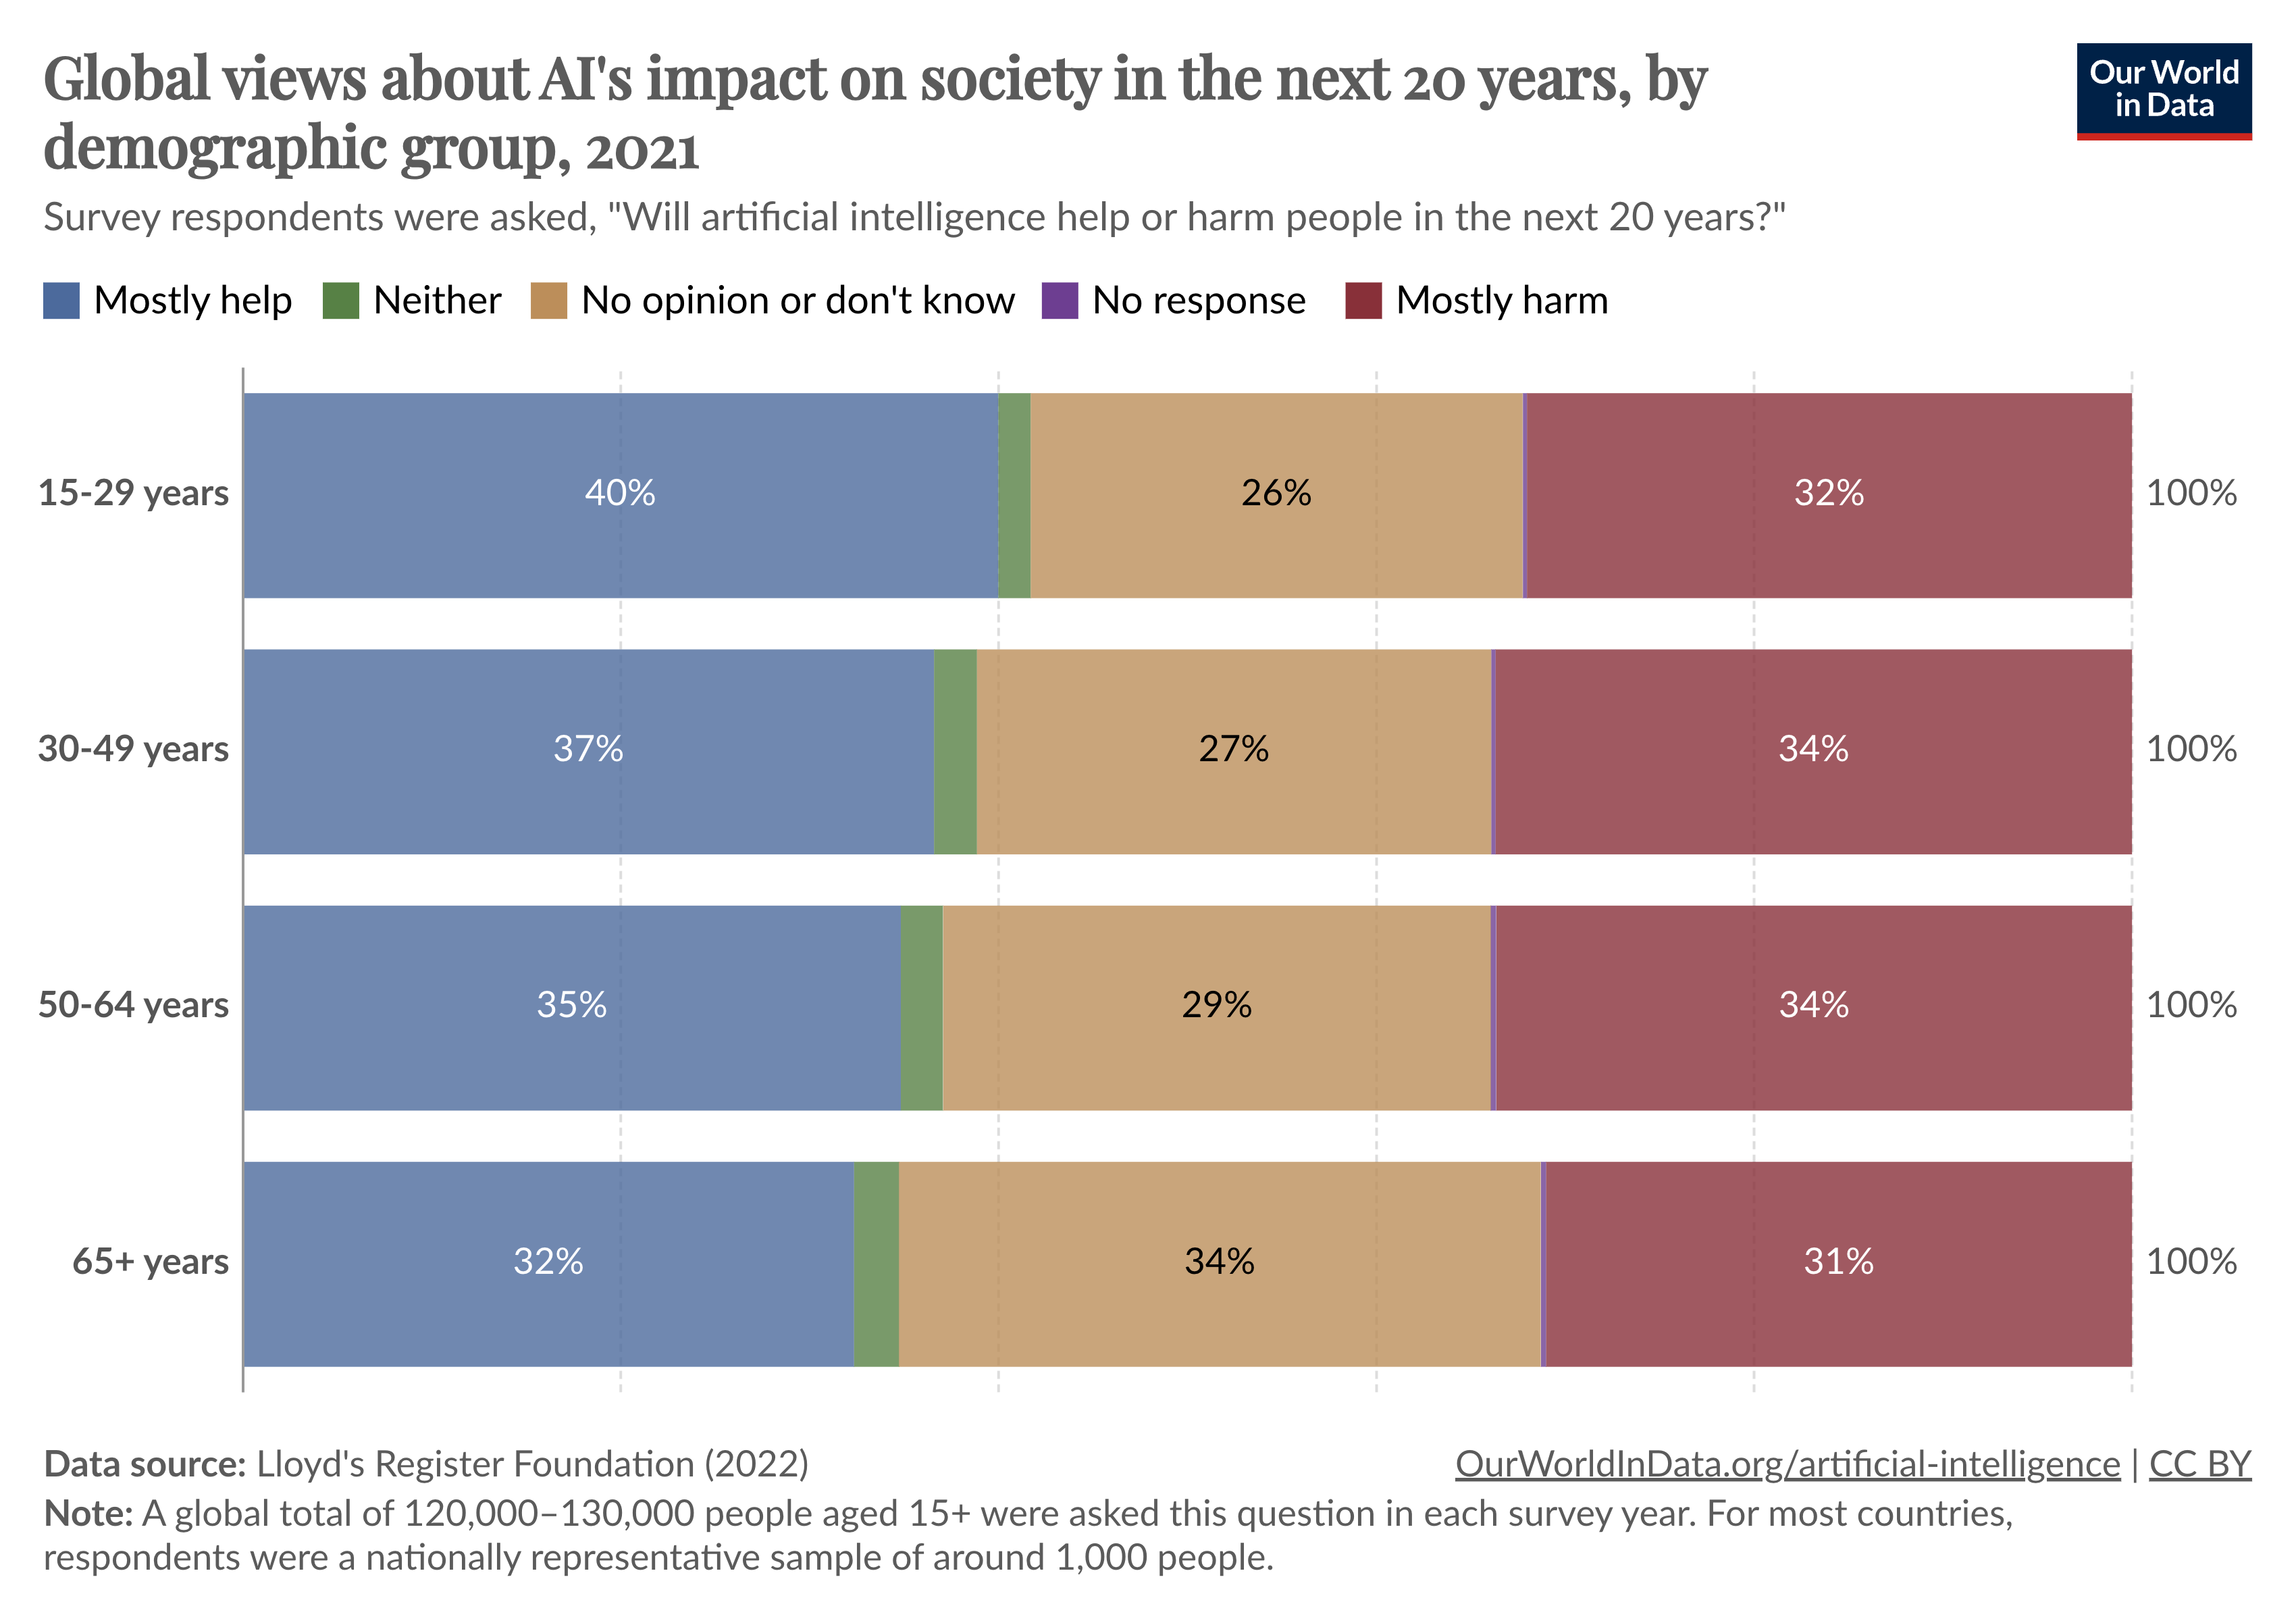
\includegraphics[width=\linewidth]{./data/influence_by_ages.png}
        \caption{Annual private investment in AI}
        \label{fig:investment}
    \end{minipage}\hfill
    \begin{minipage}[t]{0.48\linewidth}
        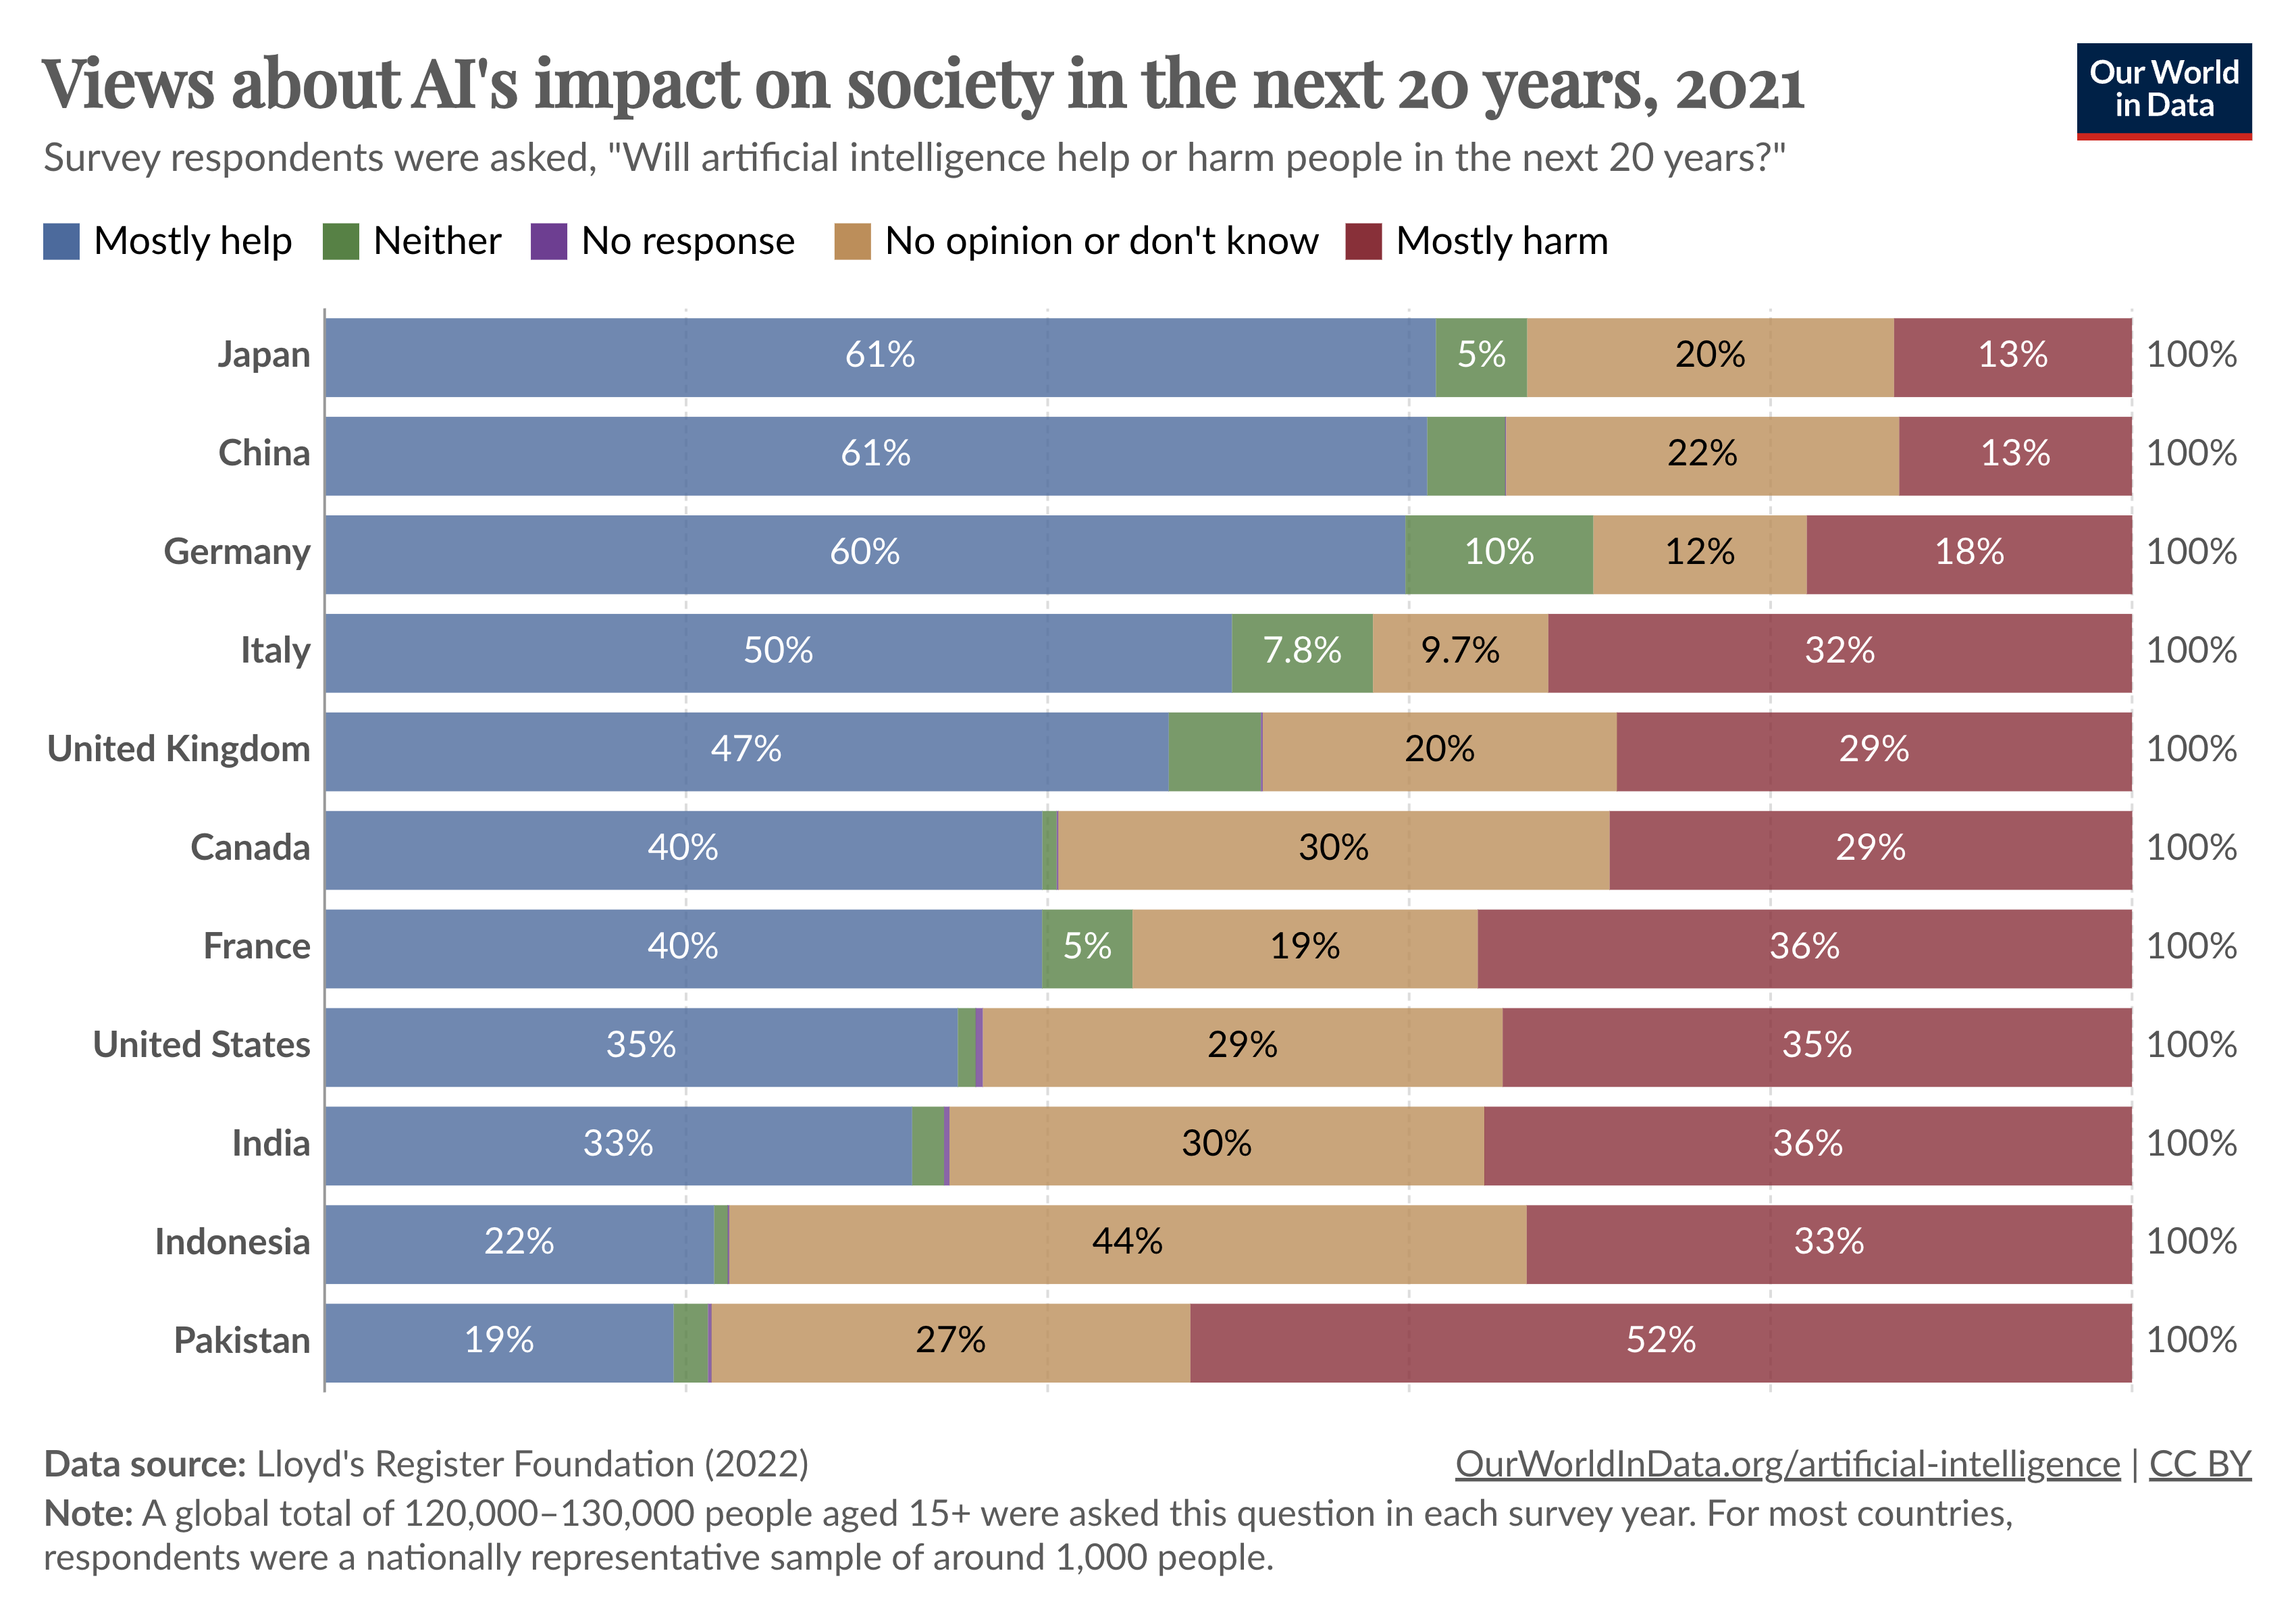
\includegraphics[width=\linewidth]{./data/influence.png}
        \caption{Views on AI's impact on society}
        \label{fig:views_ai_impact}
    \end{minipage}
\end{figure}


% 医生
\section{section2}
For doctors, doctors are in a very awkward position in the entire system. Healthcare artificial intelligence is patient-centered during its implementation.

On the one hand, artificial intelligence systems are said to be the solution for many highly skilled medical tasks 
where machines have the potential to surpass human capabilities, such as identifying normal and abnormal chest X-rays \cite{iniestaHumanRoleGuarantee2023}.
The transformative power of data technology has brought worries and fears to doctors. Machines and 
doctors seem to be placed on a double-edged balance to determine who will go and who will stay. 
They are afraid that they will be replaced by machines.
Or would disempowerment of clinicians, resulting in the development stage of HCAI, 
clinicians do not fully trust Artificial intelligen system or developers, ultimately affecting the performance of HCAI.


On the other hand, A national survey-based study in Turkey shows that most participants believed that ethical issues around data storage 
and reuse can be ignored. The perspectives of engineers and developers who create AI systems, as well as potential users (healthcare professionals) 
should be more comprehensively collected, In addition, 61.68\% of people believe that anonymity can protect privacy, 
and 70.66\% of participants believe that artificial intelligence systems do not discriminate \cite{ahunPerceptionsConcernsEmergency2023}
It is also necessary to mention its understanding of artificial intelligence ethics.




\section{section3}
(1) By educating the public and medical staff on artificial intelligence and related ethical issues, this will help 
to improve their awareness of privacy and human rights in artificial intelligence.
(2) By openly acknowledging the value of medical staff and respecting the decisions of clinicians, they realize that 
artificial intelligence is not a competitive relationship but a cooperative relationship, and the output of artificial 
intelligence is communicated to patients in a way that doctors can understand.

\section{Conclusion}
% The application potential of artificial intelligence in the medical field is huge, but in the era of artificial intelligence, 
% we should not forget that people are not just composed of data. Even when talking about personalized medicine, we should keep 
% asking ourselves: "Where are the people in AI-based personalized medicine?"
% Personhood is a profound concept related to phenomenal consciousness, intention, and free will. If clinical recommendations 
% automatically deployed by AI are directly integrated, this will preemptively prevent clinicians from developing their own clinical 
% judgment capabilities, which we humans do when developing AI tools.
% Artificial intelligence should be ensured to safeguard our health and well-being, and especially our dignity as human beings.


Artificial intelligence can do a lot in medicine, but we must remember that people are more than just data. 
Even with personalized medicine using HCAI, we need to keep asking, "Where do people fit into AI-based personalized medicine?" 
Being human involves deep ideas like awareness, purpose, and choice, which is important when we create AI tools. 
We should make sure AI helps our health and well-being, and respects our dignity as humans.



%人工智能系统的输出结果由医生以可理解的方式提供给患者。如果患者能够理解自动部署的决定是如何做出的,这就能增强患者的能力,真正实现共同决策过程,将患者作为一个整体纳入其中。


% 结论

% 人工智能不是洪水猛兽,它在以肉眼可见的速度改变着每一个人的生活方式,它的发展不可阻挡,对于政府来说要加强监管,和对人工智能方面知识的普及
% 对于医生

% 明确责任边界
% AI and advanced digital technologies are set to transform healthcare and healthcare systems in a significant way in the twenty-first century
% 3 结果:五项事实特征描述 确定了五项以人为本的事实,以描述临床医生、患者和开发人员的角色,从而确保伦理人工智能在医学中的应用。事实框架由 2.2 节中提出的问题驱动,并遵循了扩展的人工智能研究方法。2.2 节中提出的问题,并遵循 2.3 节中介绍的扩展合作模式。特别是,"事实 "旨在为以下关键问题提供答案:临床医生、患者和开发人员应发挥什么作用,才能确保人工智能在医疗保健中符合道德规范。 从 PCC 和 EBM 医学视角、协作模式和现代医疗保健需求的前景中产生的四个支柱性观点构成了 "事实 "定义的基本要素。这些基本要素如下 (i) 协作和分担责任。
% (ii) 尊重临床医生的决定。
% (iii) 对所有利益相关者进行伦理和人工智能教育。
% (iv) 赋予公民权力。



% \begin{figure}[h]
%     \centering
%     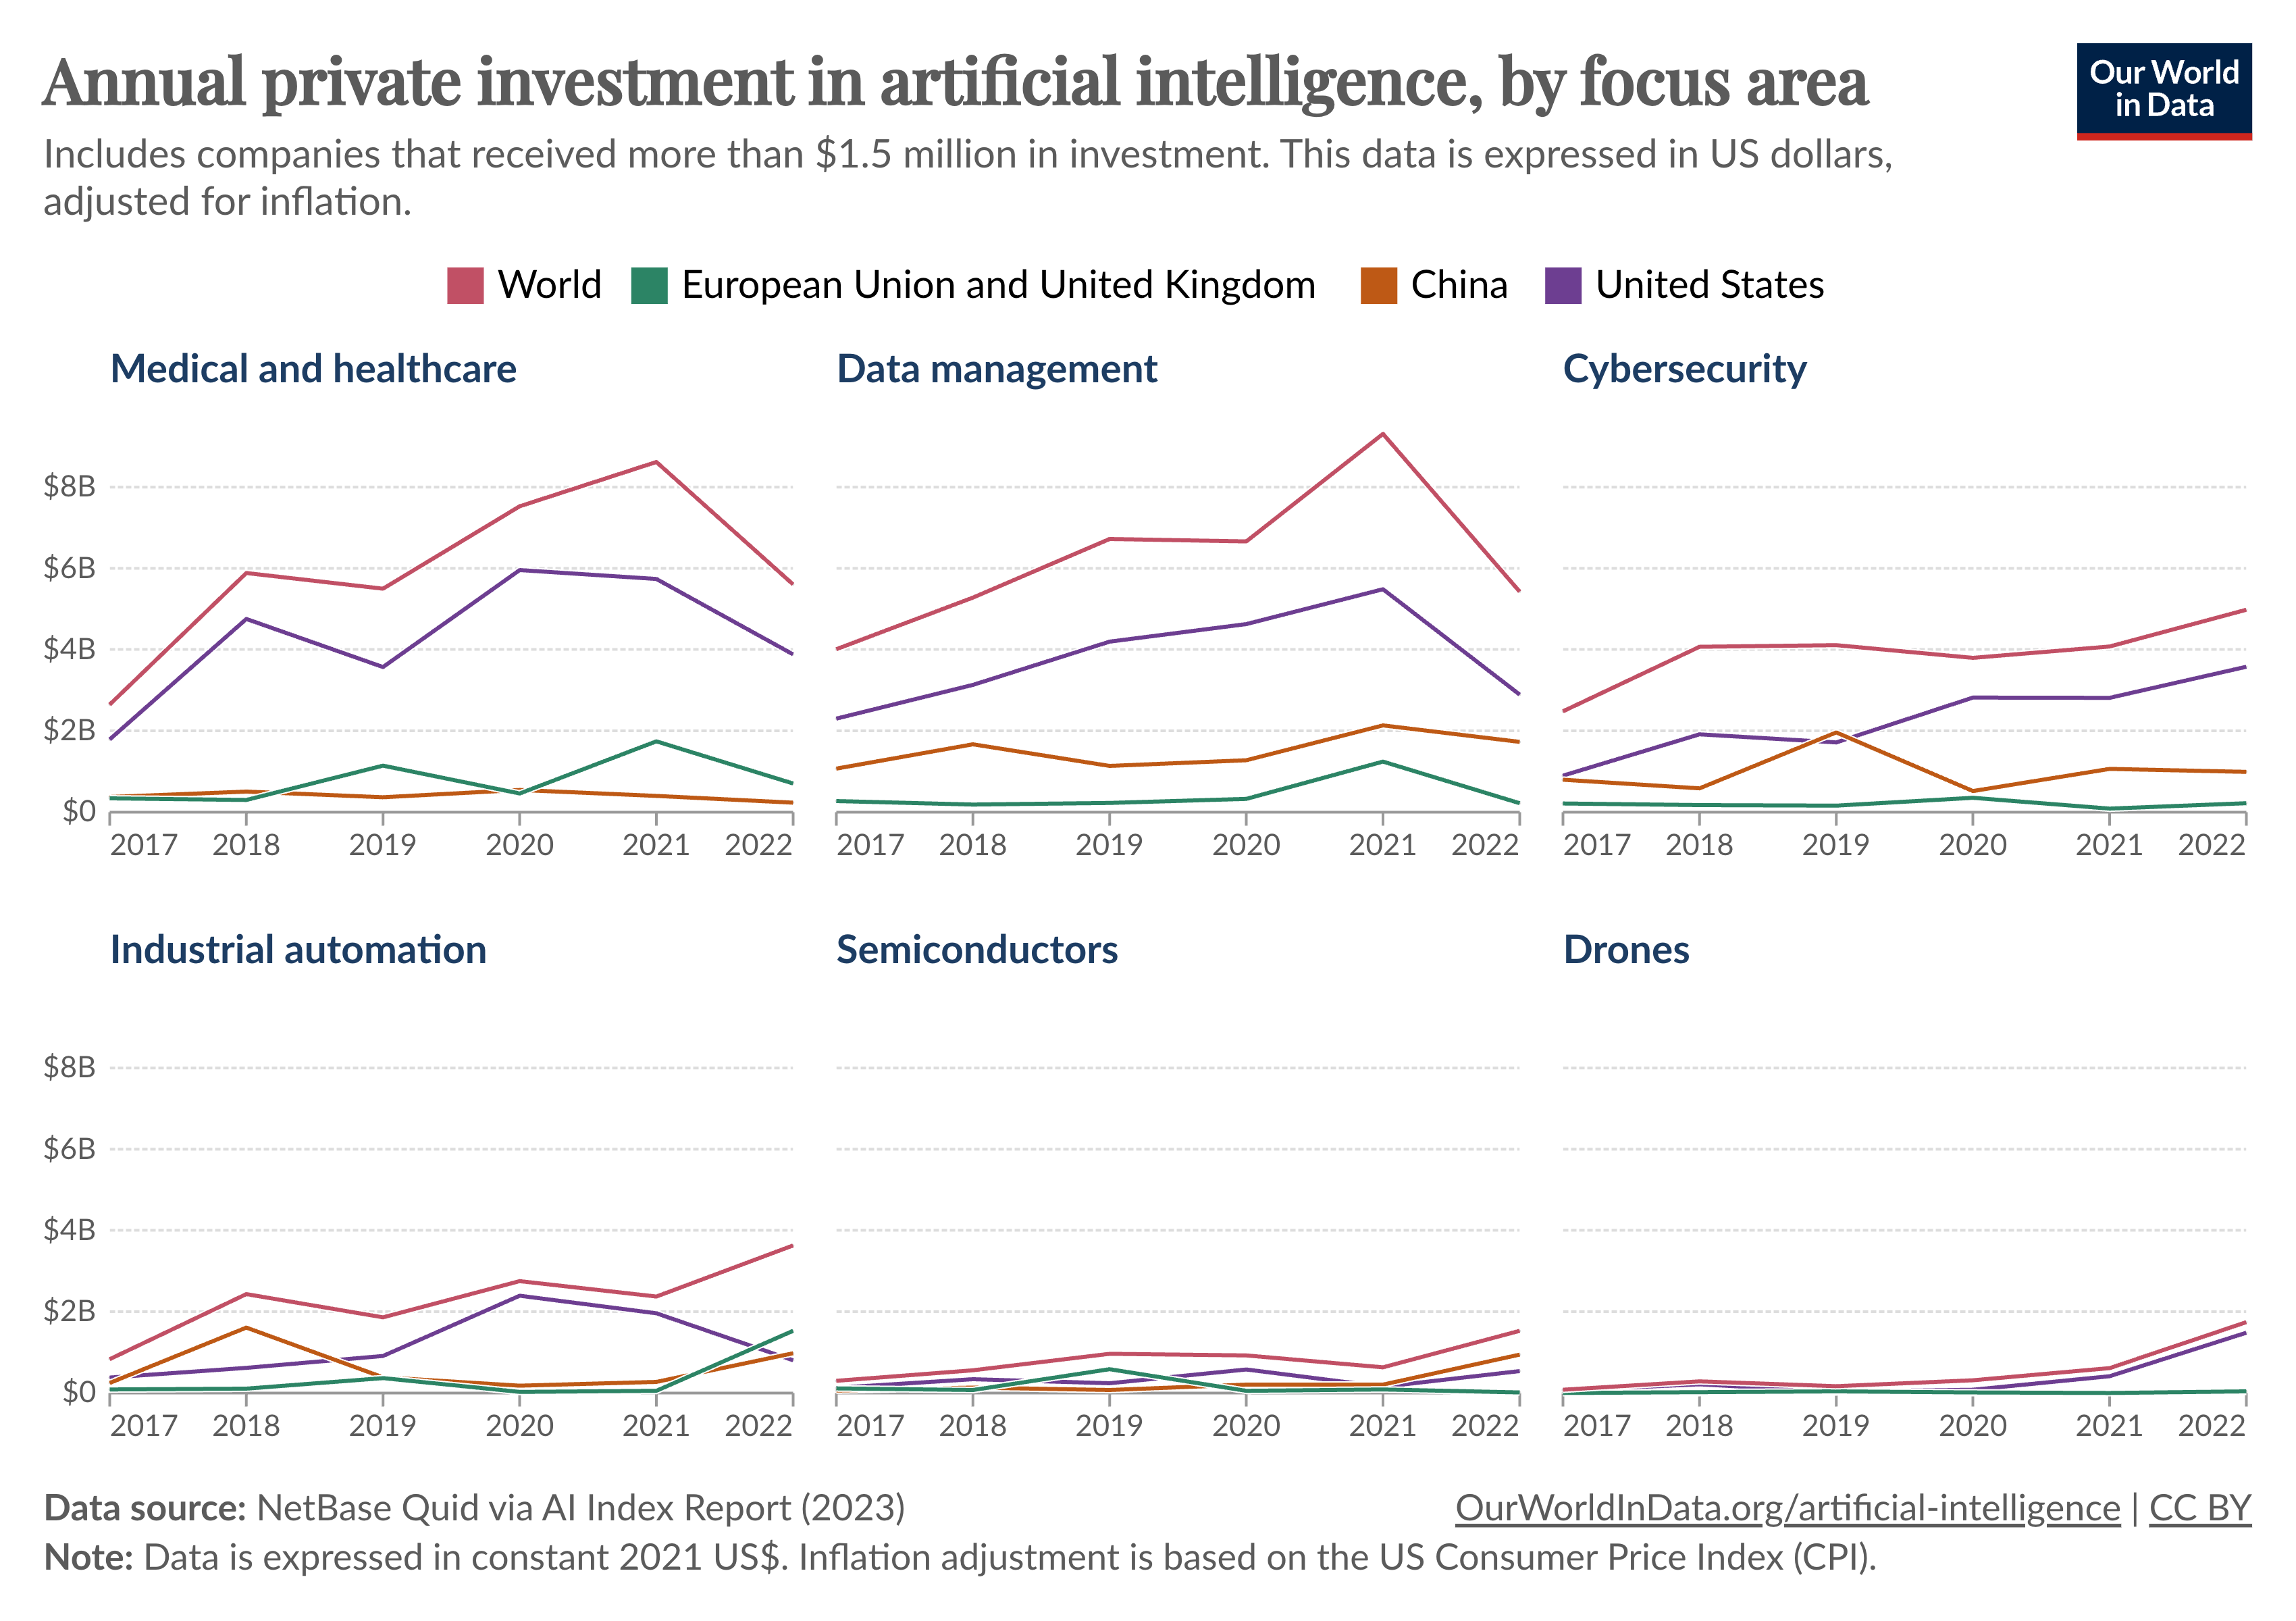
\includegraphics[width=0.9\textwidth]{./data/investegatement.png}
%     \caption{This is the title}
%     \label{fig:my_picture}
% \end{figure}



% \begin{figure}[h]
%     \centering
%     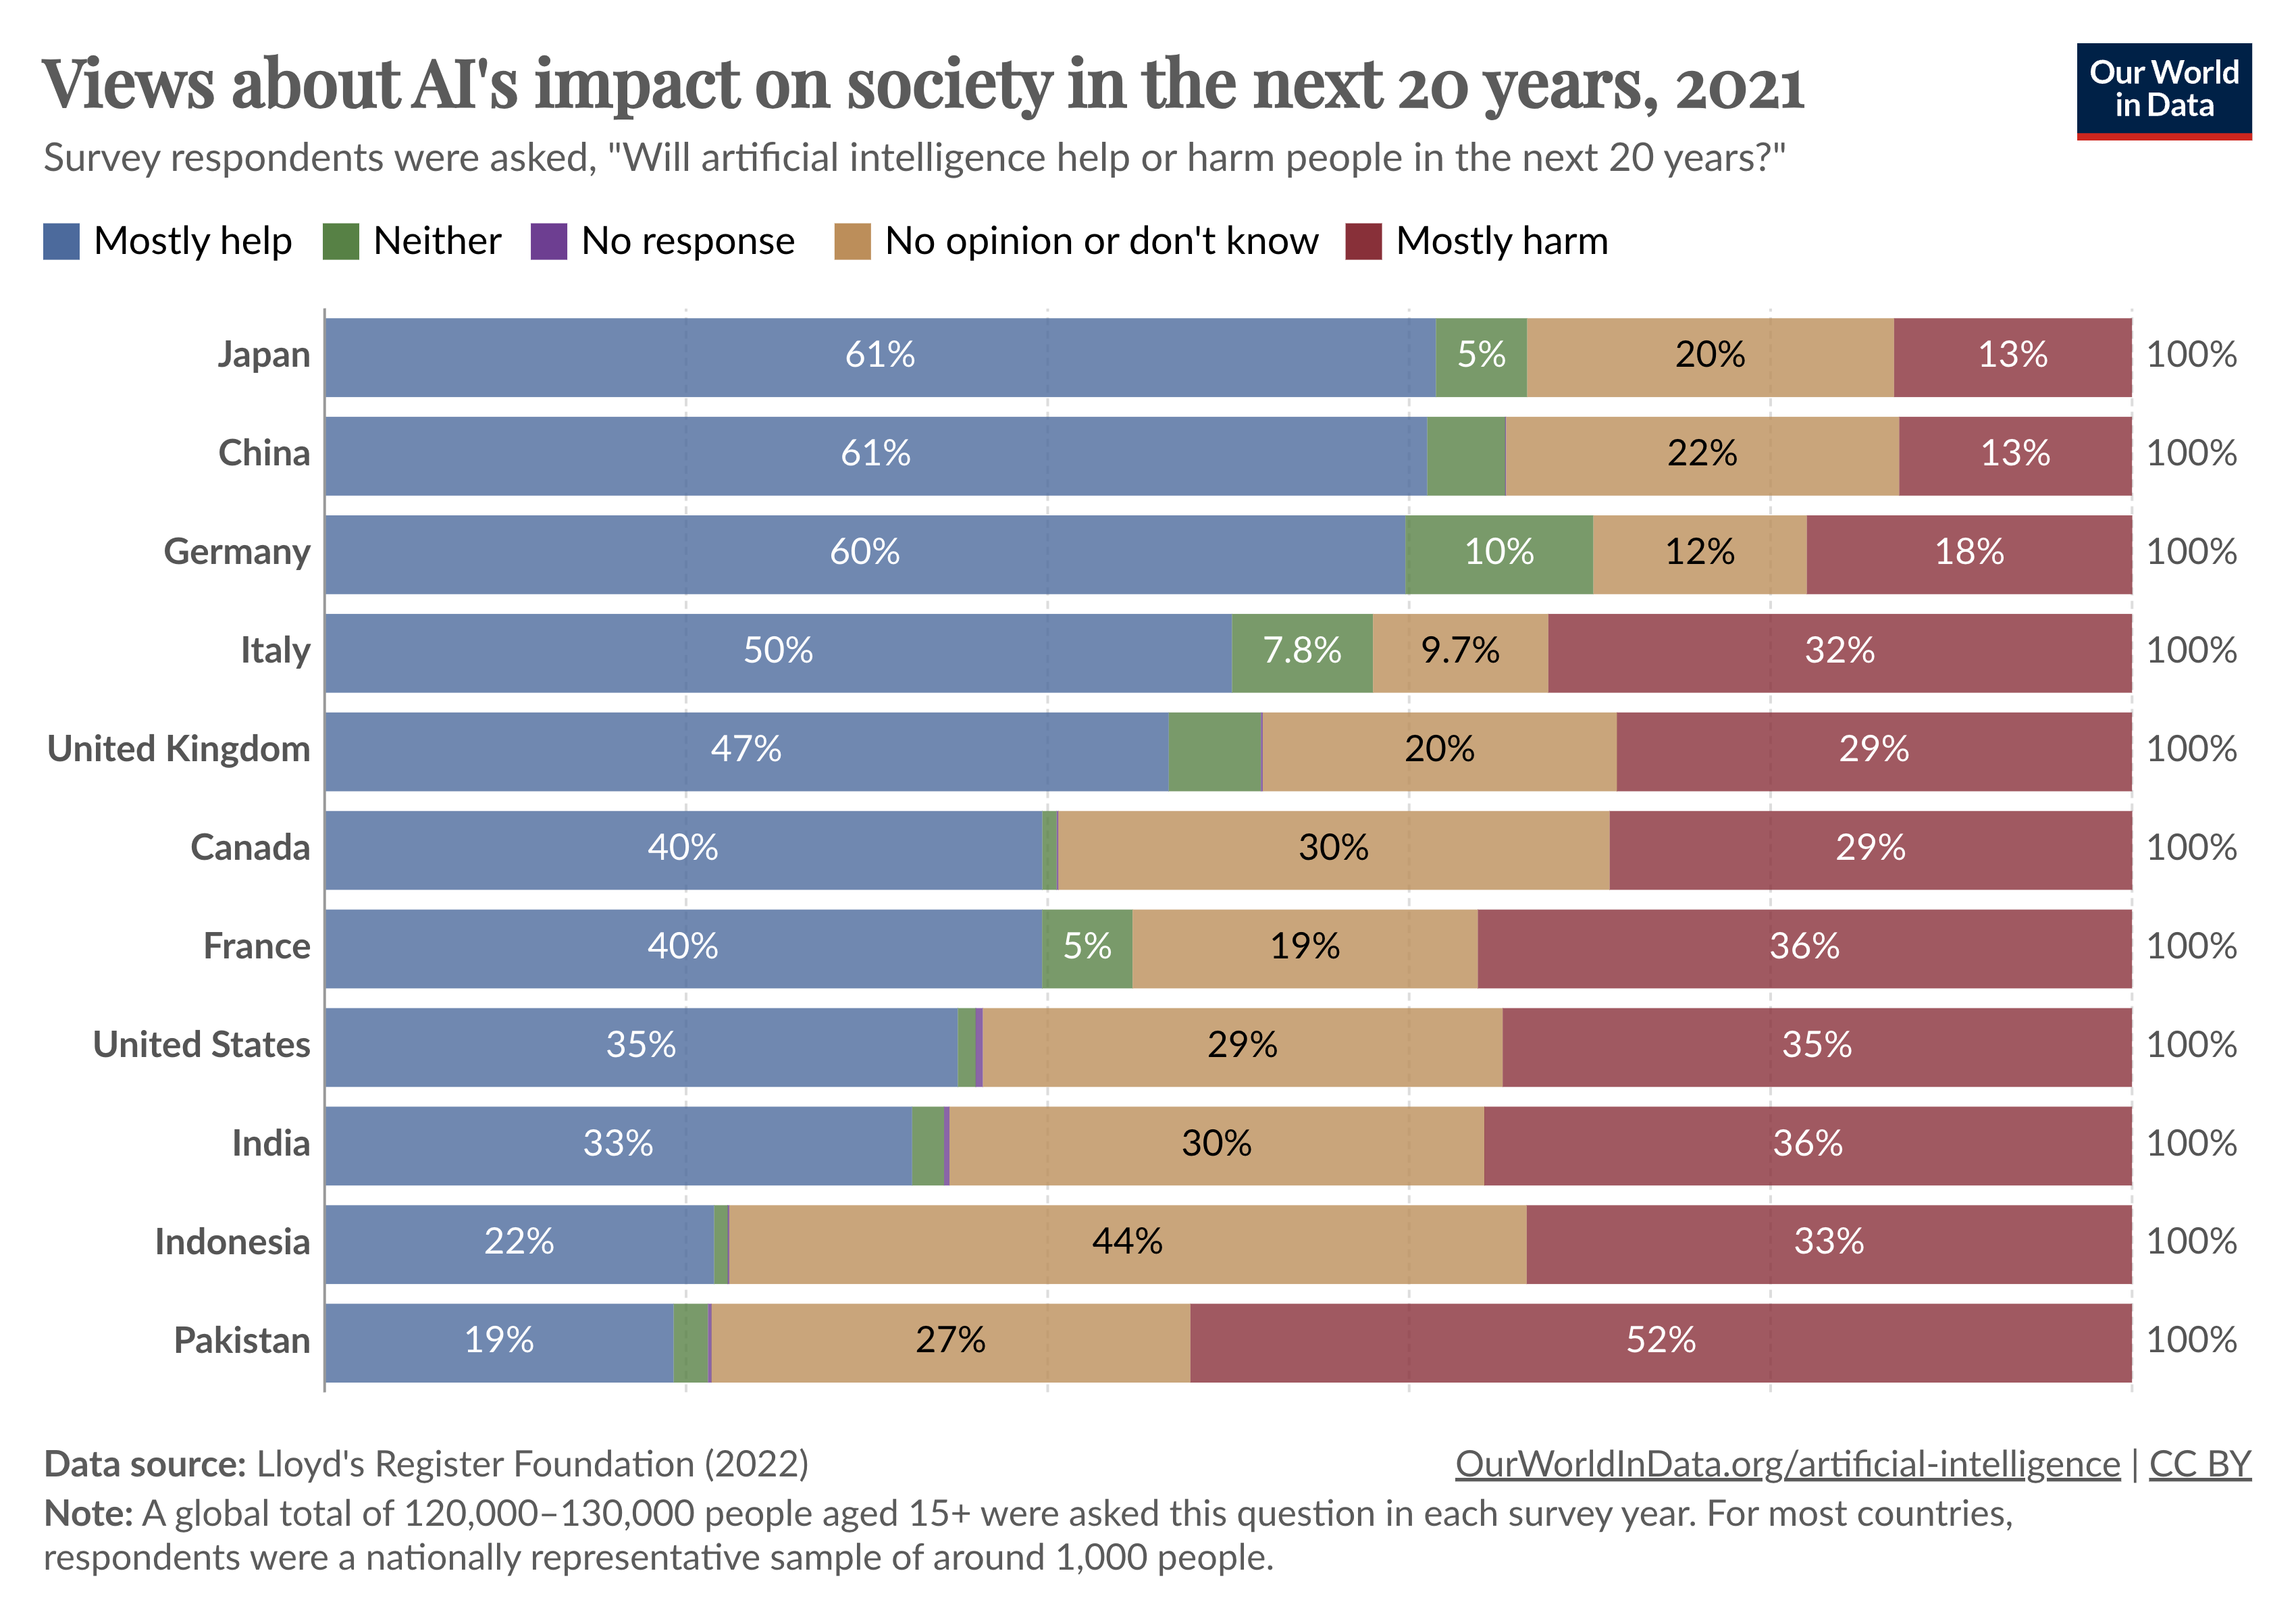
\includegraphics[width=0.9\textwidth]{./data/influence.png}
%     \caption{This is the title}
%     \label{fig:my_picture}
% \end{figure}
















%----------------------------------------------------------------------------------------

\bibliographystyle{unsrt} % This specifies the style of the bibliography
\bibliography{/Users/dengkai/workspace/papers/latex/config/ref} % This should match the name of your .bib file without the extension


\end{document}

